\chapter{Oracle Aplication Express}

\section{Pengenalan Oracle APEX}

Oracle Aplication Express\cite{OracleApex} yang disebut juga HTML-DB adalah sebuah framework yang berbasis pada sebuah database dedicated (sementara ini sampai versi terbaru masih dedicated untuk Oracle DB. Oracle APEX Adalah sebuah wadah dan sarana untuk membuat aplikasi yang menggunakan database Oracle Itu sendiri, pada kelas Online pertama saya belajar banyak hal cara Menggunakan Aplikasi Oracle Apex online yang di dalam video sudah diberikan link diantaranya Request Workspace, Create Workspace, Membuat Spreadsheet Pertama.

\section{Tahapan Pembuatan Aplikasi Oracle Apex}
Langkah pertama yang harus dilakukan adalah membuka website https://apex.oracle.com, disini kita akan mendapatkan akses untuk memasuki Oracle Apllication Express, pastikan email yang dimasukkan valid untuk membuat Workspace, berikut adalah langkah langkah pembuatan Aplikasi pada Oracle APEX :

\begin{enumerate}
\item[1]Pergi ke Website Oracle APEX, https://apex.oracle.com, lalu klik Get Start For Free.

\begin{figure}[!htbp]

    \begin{center}
        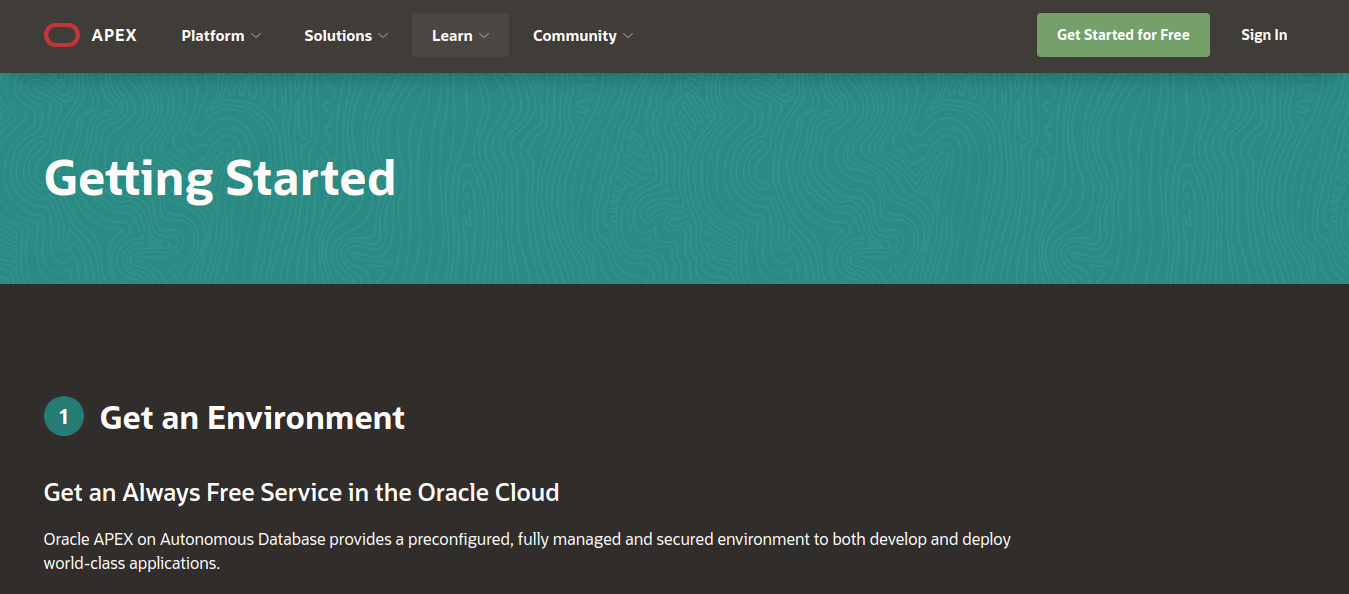
\includegraphics[scale=0.2]{figures/TampilanAracleApex.png}
        \caption{\textit{Go to Website Get Start For Free.}}
        \end{center}   
        \end{figure}
        \begin{figure}[!htbp]
\item[2]Klik Request a Free Worksace.

    \begin{center}
    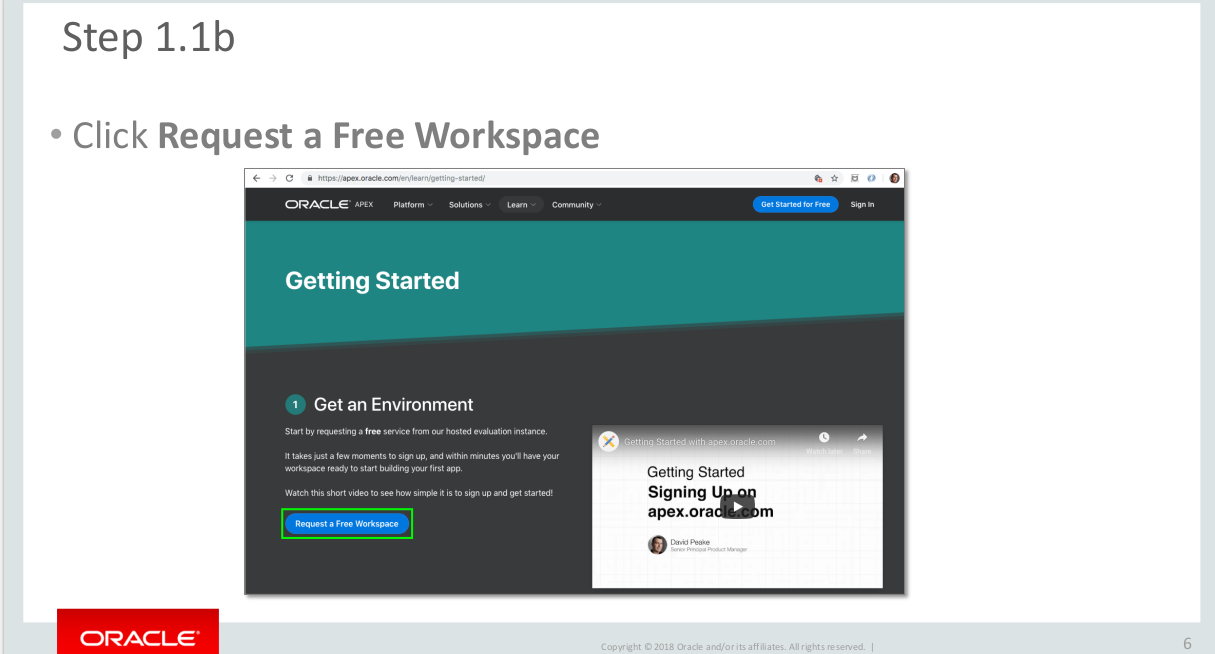
\includegraphics[scale=0.2]{figures/step1.png}
    \caption{\textit{Request A Free Workspace.}}
    \end{center}

\item[3]Isikan data diri anda seperti nama,email,dan workspace.

        
\item[4]Centang apakah anda pernah melakukan hal tersebut lalu next.  

      
\item[5]Isikan pada kolom tersebut bebas, mengapa anda ingin menggunakan layanan ini ?, lalu klik next.

 
\item[6] Centang Accept, lalu klik next.


\item[7] Tahapan terakhir untuk mengkonfirmasi apakah ini anda, lalu klik next.

   
\item[8] Workspace Sukses Dibuat dan Cek Email.

    \begin{center}
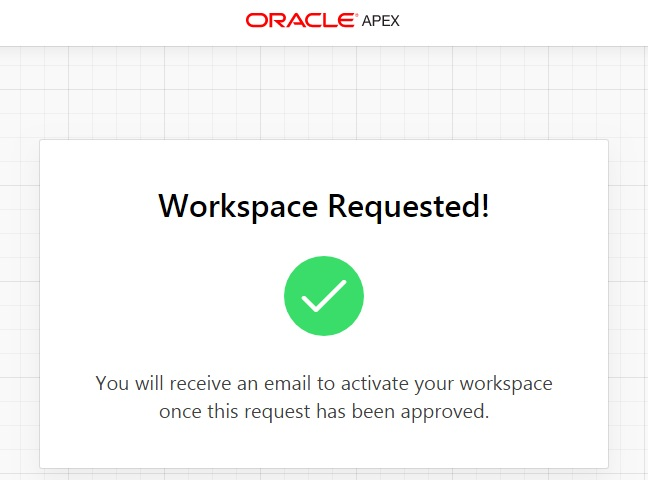
\includegraphics[scale=0.5]{figures/pict(3).jpg}
    \caption{\textit{Finish lalu Cek Email}}
        \end{center}
\label{gambar}
\end{figure}

\begin{figure}
\item[9] Workspace yang dibuat telah di Acc lalu klik continue.

    \begin{center}
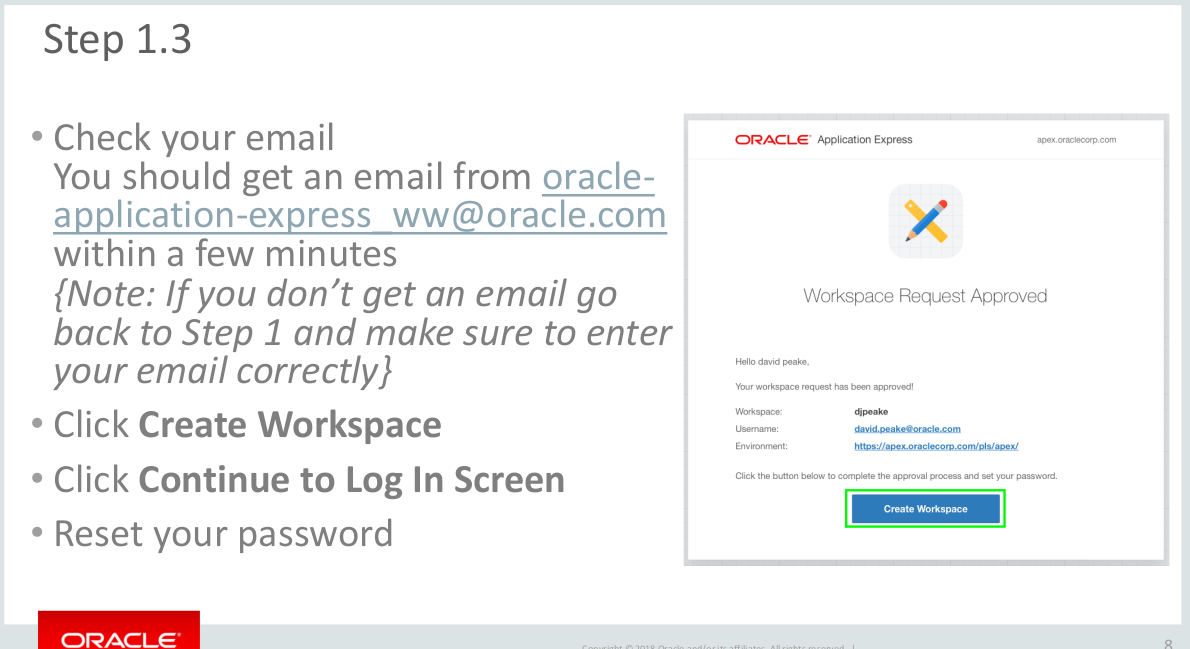
\includegraphics[scale=0.2]{figures/step2.png}
    \caption{\textit{Email Acc.}}
        \end{center}
\label{gambar}
\end{figure}




\begin{figure}
\item[10] sekarang kita masuk ke tampilan halaman awal aplikasi Oracle Express.

    \begin{center}
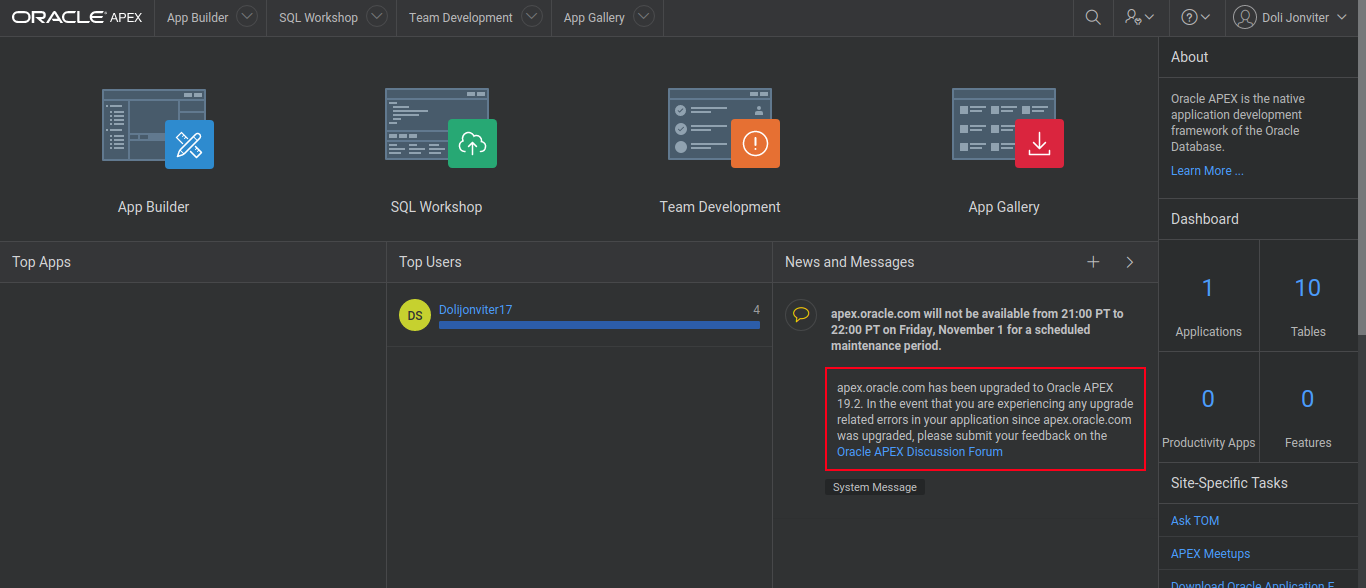
\includegraphics[scale=0.3]{figures/halamanApex.png}
    \caption{\textit{Oracle Apex Home.}}
        \end{center}
\label{gambar}
\end{figure}

\begin{figure}
\item[11] Buka App Builder lalu klik Create New App.

    \begin{center}
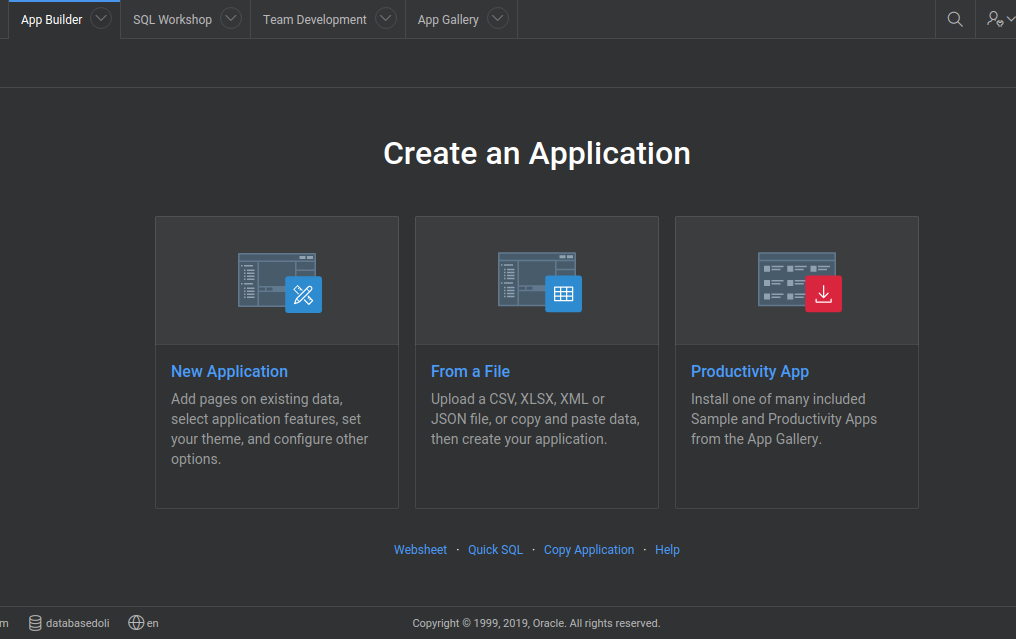
\includegraphics[scale=0.4]{figures/createAppFromfile.png}
    \caption{\textit{Oracle Apex App Builder}}
        \end{center}
\label{gambar}
\end{figure}

\begin{figure}
\item[12] Klik Copy and Paste, pada select data CSV atau Sample Data Set pilih Project and Tables lalu next.

    \begin{center}
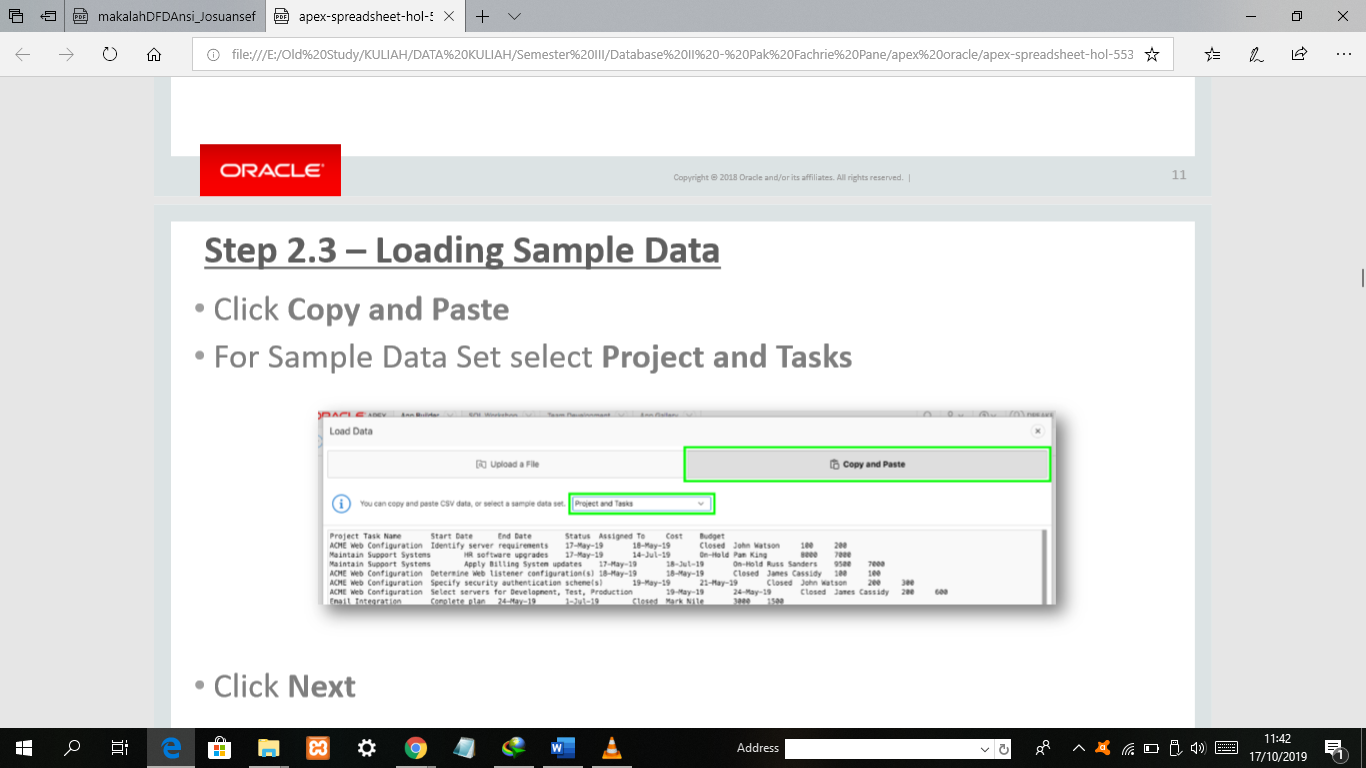
\includegraphics[scale=0.2]{figures/pict(9).png}
    \caption{\textit{Sample Data Set/ Select data CSV}}
        \end{center}
\label{gambar}
\end{figure}

\begin{figure}
\item[13] Memilih Sampel Data untuk digunakan

    \begin{center}
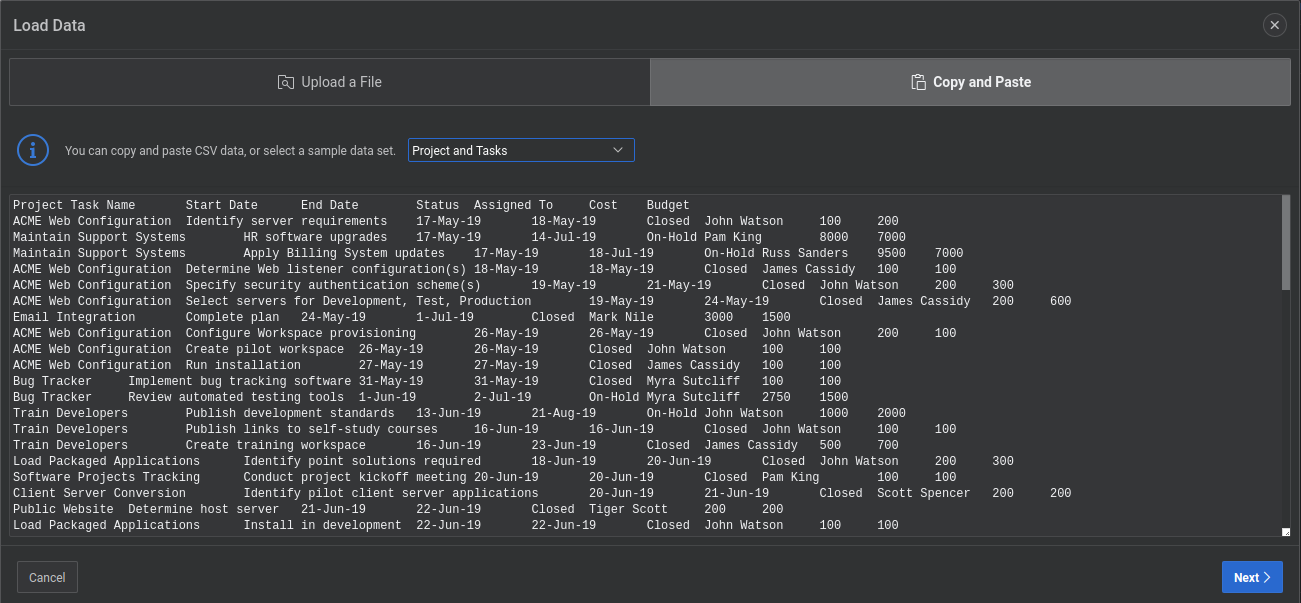
\includegraphics[scale=0.3]{figures/sampelData.png}
    \caption{\textit{Load Data.}}
        \end{center}
\label{gambar}
\end{figure}

\begin{figure}
    \begin{center}
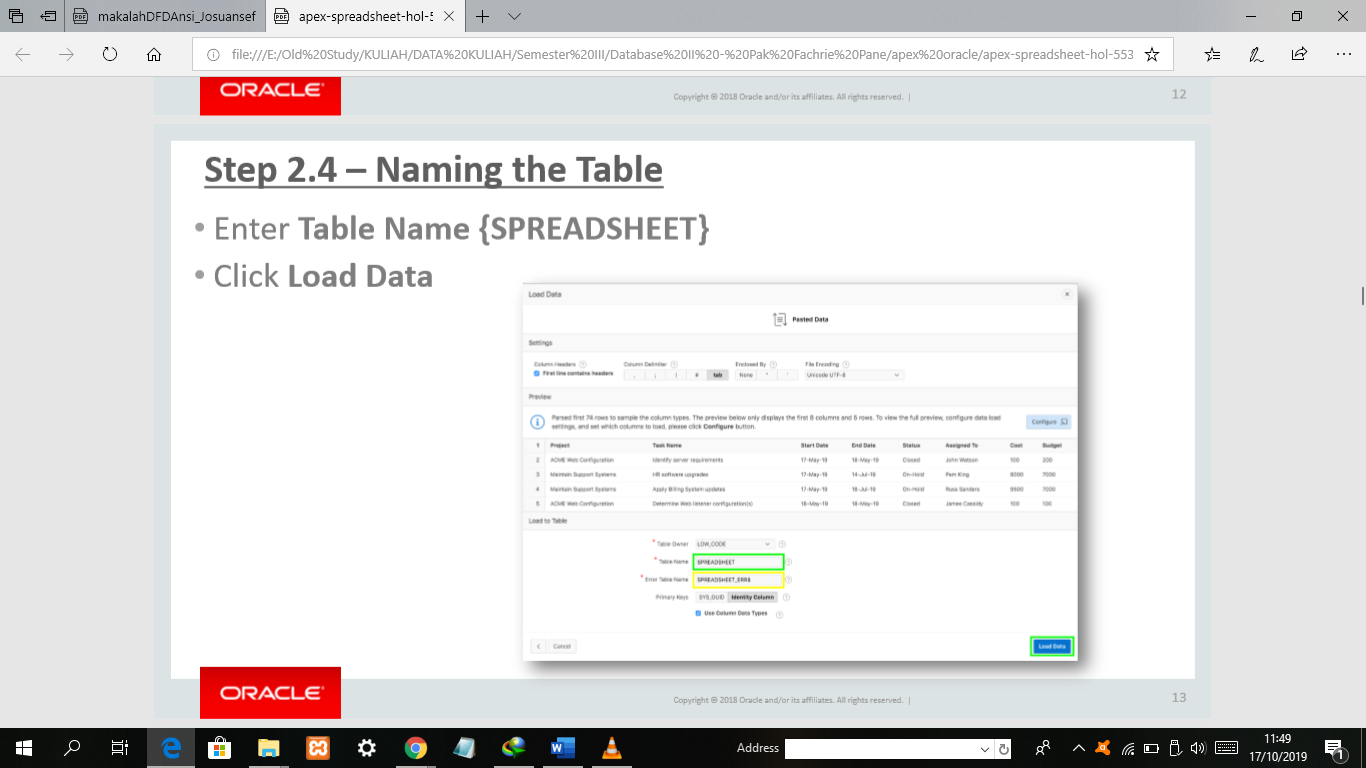
\includegraphics[scale=0.2]{figures/pict(11).png}
    \caption{\textit{Load Data 2}}
        \end{center}
\label{gambar}
\end{figure}

\begin{figure}
\item[14] Load Data Sukses , klik Continue to Create Aplication Wizard.

    \begin{center}
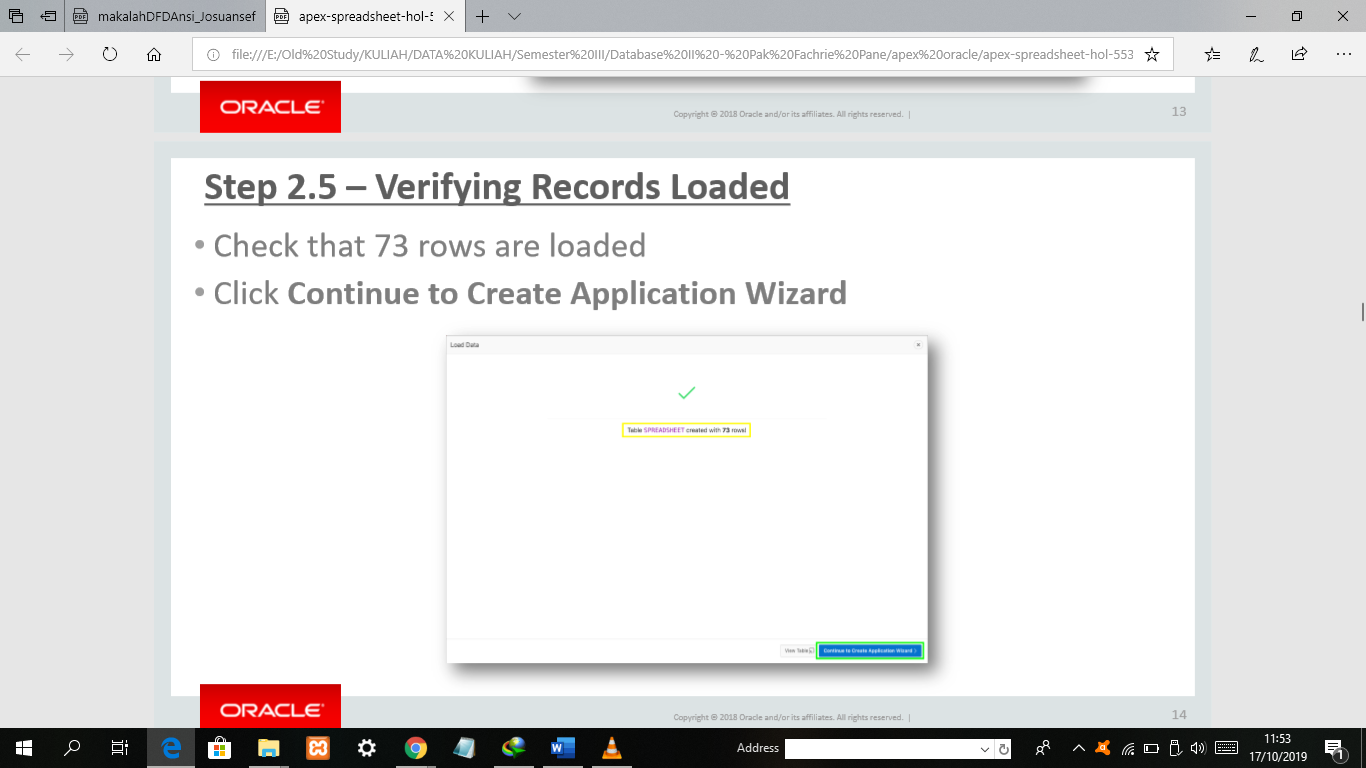
\includegraphics[scale=0.2]{figures/pict(12).png}
    \caption{\textit{Oracle Apex Load Data Success.}}
        \end{center}
\label{gambar}
\end{figure}


\begin{figure}
\item[15]Create Application .

    \begin{center}
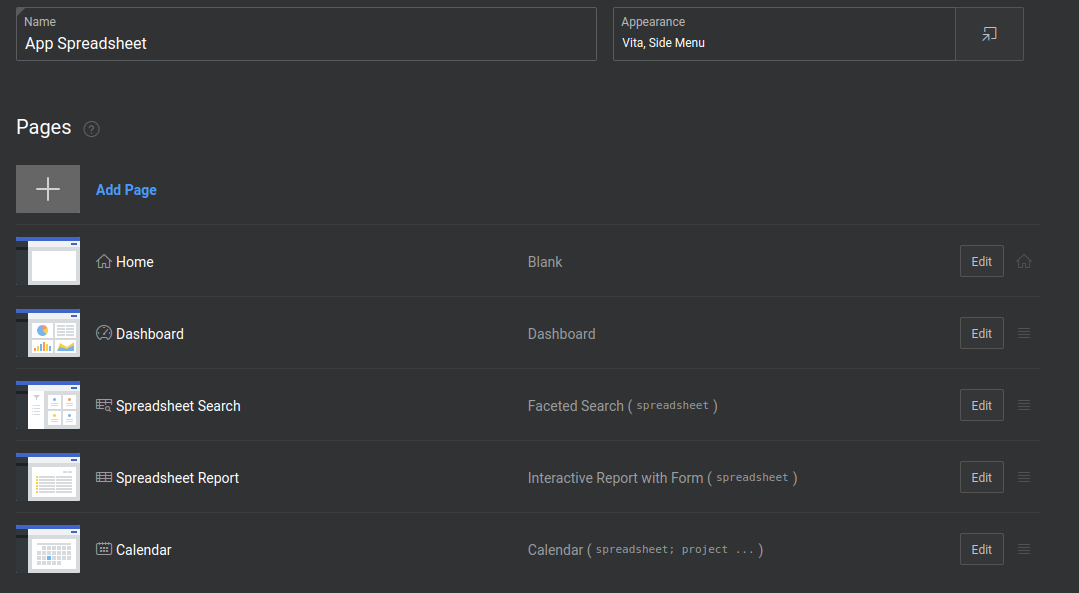
\includegraphics[scale=0.4]{figures/gambar5.png}
    \caption{\textit{Create an Application}}
        \end{center}
\label{gambar}
\end{figure}

\begin{figure}
\item[16]Create Sample Data dari Oracle Apex.

    \begin{center}
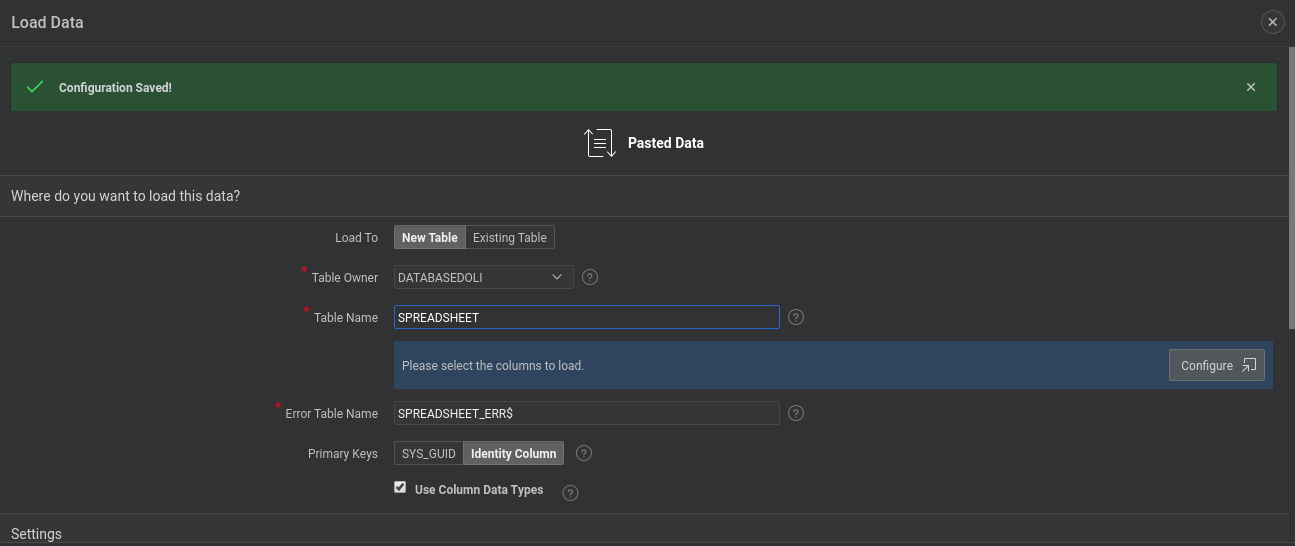
\includegraphics[scale=0.3]{figures/creatSampleData.png}
    \caption{\textit{Loading Data}}
        \end{center}
\label{gambar}
\end{figure}

\begin{figure}
\item[17]Setelah selesai mengimport file dan membuat nama tabel maka aplikasi akan melakukan running untuk menuju halaman login .

    \begin{center}
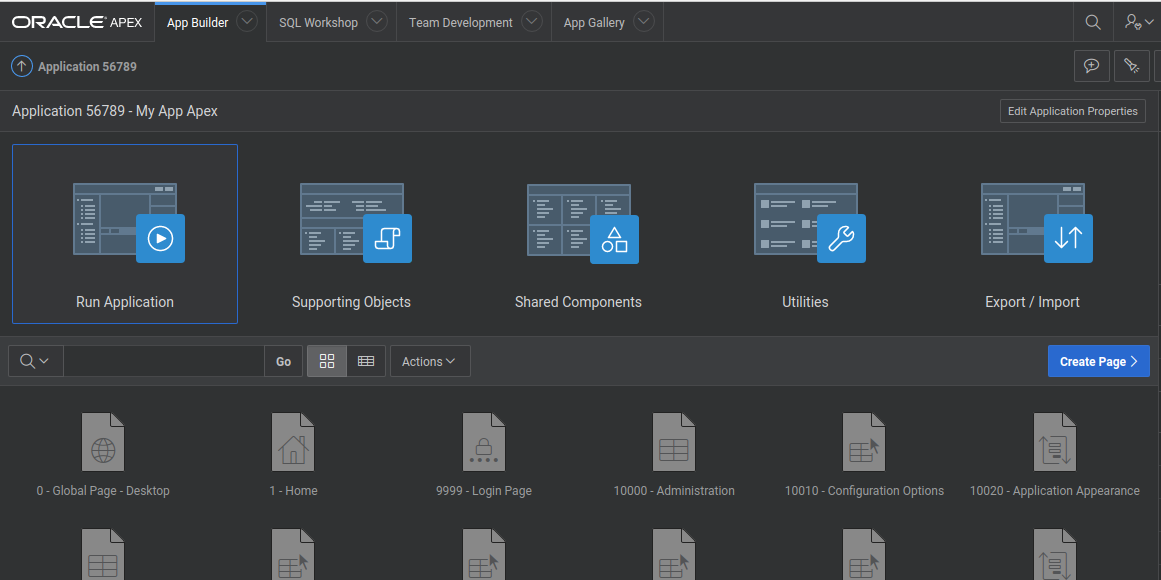
\includegraphics[scale=0.4]{figures/tampilaApp.png}
    \caption{\textit{App Builder Success}}
        \end{center}
\label{gambar}
\end{figure}

\begin{figure}
\item[18]Login untuk melihat aplikasi yang sudah dibuat sebelumnya.

    \begin{center}
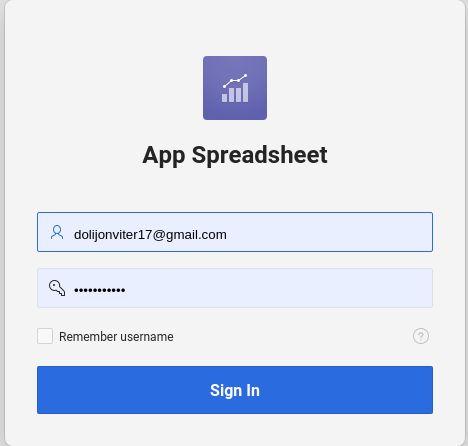
\includegraphics[scale=0.4]{figures/tampilLogin.png}
    \caption{\textit{Sign In Spreadsheet}}
        \end{center}
\label{gambar}
\end{figure}

\begin{figure}
\item[19]Hasil Akhir.

    \begin{center}
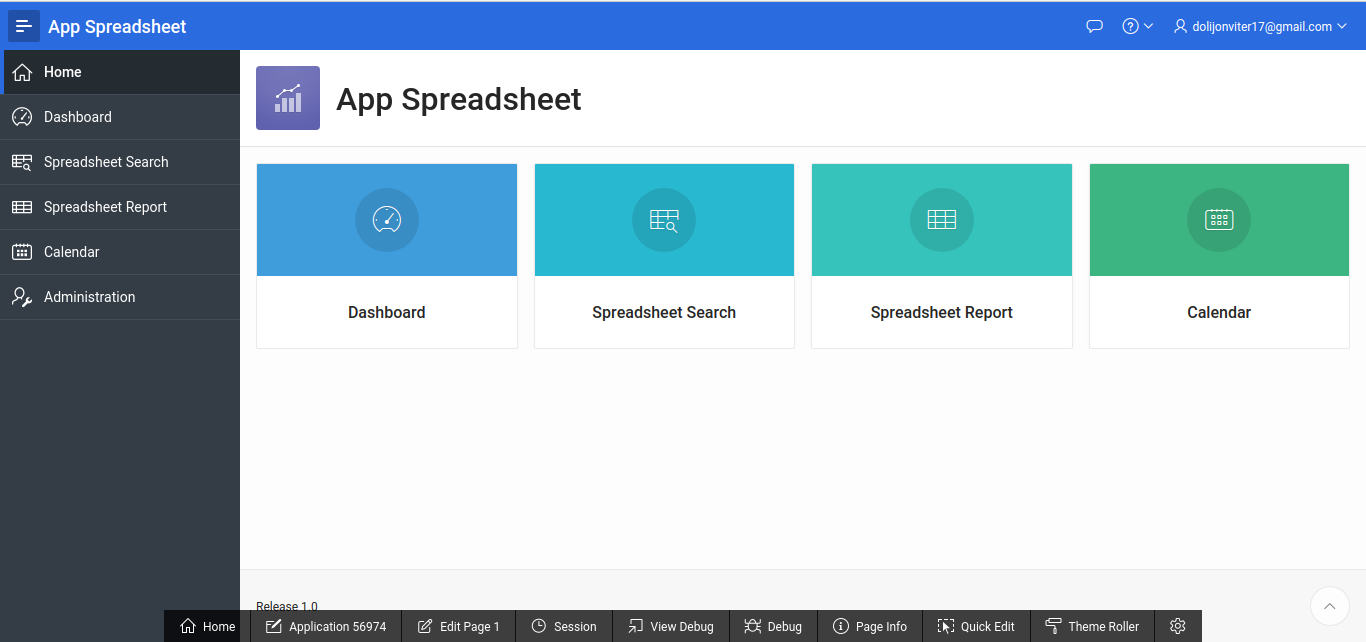
\includegraphics[scale=0.3]{figures/hasilAkhir.png}
    \caption{\textit{Welcome Spreadsheet}}
        \end{center}
\label{gambar}
\end{figure}

\end{enumerate}
